\subsection{Testing}

This time, we have to build up a knowledge base, and check the the proposed hypothesis is entailed from the knowledge base. Like before, we will start by a trivial test, checking if the proposition 'a' is entailed by a knowledge base consisting of the clause 'a'. We expect the proof to be successful. This matches the actual output, as seen in figure \ref{fig:RPtest1}.

\begin{figure}[H]
    \centering
    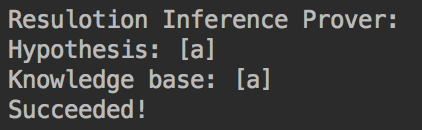
\includegraphics[width=0.3\linewidth]{ResolutionProver/RPtest1.png}
    \caption{Trivial refutation proof test result.}
    \label{fig:RPtest1}
\end{figure}

Next we test an implication in CNF. The example here contains 'not a or b' in the knowledge base, and 'a' as the hypothesis, and we wish to see if it entails 'b'. This matches the actual output, as seen in figure \ref{fig:RPtest2}.

\begin{figure}[H]
    \centering
    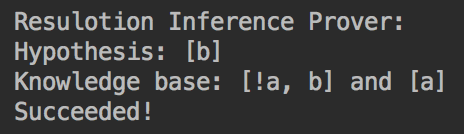
\includegraphics[width=0.3\linewidth]{ResolutionProver/RPtest2.png}
    \caption{Refutation proof for implication test result.}
    \label{fig:RPtest2}
\end{figure}

Finally we want to test if it correctly identifies when something is not entailed by the knowledge base. The example here contains 'a or b' in the knowledge base and 'a' as the hypothesis. We expect this to be 'not proven', as the knowledge base does not contain enough enough information to entail the hypothesis. This matches with the actual output, as seen in figure \ref{fig:RPtest3}.

\begin{figure}[H]
    \centering
    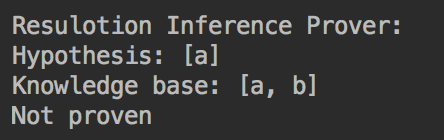
\includegraphics[width=0.3\linewidth]{ResolutionProver/RPtest3.png}
    \caption{Refutation proof where hypothesis does not entail from the knowledge base.}
    \label{fig:RPtest3}
\end{figure}

Based on these tests, it is probable that the implementation of the inference engine for propositional logic is correct,as it has satisfied our behavioral expectations.